%        File: eyeStand_cardboard.tex
%     Created: Mon Apr 06 11:00 am 2020 C
% Last Change: Mon Apr 06 11:00 am 2020 C
%


\documentclass[a4paper]{article}
\usepackage{subcaption}
\usepackage[utf8]{inputenc}
\usepackage{tikz}
\usepackage[left=2.5cm,top=3cm,right=2.5cm,bottom=3cm,bindingoffset=0.5cm]{geometry}


\begin{document}
\title{eyeStand: Cardboard \\ Instructions and schematic}
\author{}

\maketitle

eyeStand is a simple design intended to help lecturers and instructors with online courses. It is a simple construction to help anyone stream handwritten text while teaching online.

The following are some pictures of the cardboard version of eyeStand. 

\begin{figure}[h!]
  \centering
  \begin{subfigure}[b]{0.4\linewidth}
    \includegraphics[width=\linewidth]{empty.jpg}
    \caption{Overall design}
  \end{subfigure}
  \begin{subfigure}[b]{0.4\linewidth}
    \includegraphics[width=\linewidth]{homeview_used.jpg}
    \caption{Intended use}
  \end{subfigure}
  \begin{subfigure}[b]{0.4\linewidth}
    \includegraphics[width=\linewidth]{topused.jpg}
    \caption{Intended use (top) }
  \end{subfigure}
  \caption{eyeStand with usage example}
  \label{fig:coffee}
\end{figure}

The height and the width of this design has been tested to work with several diffent older models of smartphones and standard A4 sheets. The construction is very sturdy so that your phone is safe and secure.


\begin{figure}[htp]
\begin{center}
\definecolor{qqqqff}{rgb}{0.0,0.0,1.0}
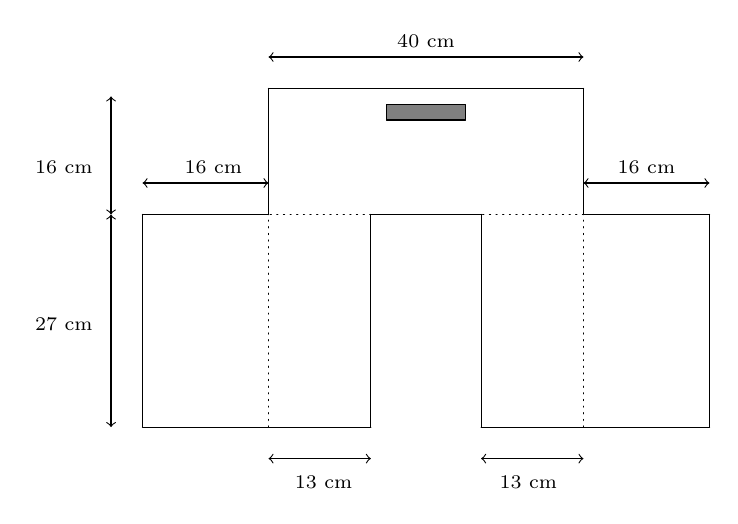
\begin{tikzpicture}[line cap=round,line join=round,x=1.0cm,y=1.0cm]
\begin{scriptsize}
  
\draw (0,0)[dotted]--(0,2.7);
\draw (0,0)--(1.3,0);
\draw (0,-0.4)[<->]--(1.3,-0.4);
\draw (2.7,-0.4)[<->]--(4.0,-0.4);
\draw (1.3,0)--(1.3,2.7);
\draw (2.7,0)--(4.0,0);
\draw (2.7,0)--(2.7,2.7);
\draw (4,0)[dotted]--(4,2.7);
\draw (4,2.7)[dotted]--(2.7,2.7); 
\draw (1.3,2.7)[dotted]--(0,2.7);
\draw (1.3,2.7)--(2.7,2.7);
\draw (0,2.7)--(0,4.3);
\draw (0,4.3)--(4.0,4.3);
\draw (4.0,4.3)--(4.0,2.7);
\draw (4.0,2.7)--(5.6,2.7);
\draw (5.6,2.7)--(5.6,0);
\draw (5.6,0)--(4.0,0);
\draw (5.6,3.1)[<->]--(4.0,3.1);
\draw (0,3.1)[<->]--(-1.6,3.1);
\draw (0,0)--(-1.6,0);
\draw (-1.6,2.7)--(-1.6,0);
\draw (-2.0,2.7)[<->]--(-2.0,4.2);
\draw (-1.6,2.7)--(0,2.7);
\draw (-2,0)[<->]--(-2,2.7);
\draw (0,4.7)[<->]--(4.0,4.7);
\draw[color=black] (-2.6, 1.3 ) node {27 cm};
\draw[color=black] (-2.6, 3.3 ) node {16 cm};
\draw[color=black] (-0.7, 3.3 ) node {16 cm};
\draw[color=black] (4.8, 3.3 ) node {16 cm};
\draw[color=black] (2.0, 4.9 ) node {40 cm};
\draw[color=black] (0.7, -0.7 ) node {13 cm};
\draw[color=black] (3.3, -0.7 ) node {13 cm};
\draw[gray,fill] (1.5,3.9) rectangle ++(1.0,0.2);
\draw[draw = black] (1.5,3.9) rectangle ++(1.0,0.2);

% \draw[color=black] (-3,0) node {$\triangleleft$};
%\draw[color=black] (-2,1) node {$\triangledown$};
%\draw[color=black] (-0.8,2.2) node {$(w, \textcolor[rgb]{0.0,0.0,1.0}{-l+1},\textcolor[rgb]{1.0,0.0,0.0}{k})$};
%\draw[color=black] (-2.2,1.2) node {$(w, \textcolor[rgb]{0.0,0.0,1.0}{-l},\textcolor[rgb]{1.0,0.0,0.0}{k-1})$};
\end{scriptsize}
\end{tikzpicture}
\\
\begin{tikzpicture}[line cap=round,line join=round,x=1.0cm,y=1.0cm]
  \begin{scriptsize}
\draw (0,0)--(4.0,0);
\draw (0,0)--(0.0,1.5);
\draw (4.0,0)--(4.0,1.5);
\draw (0.0,1.5)--(4.0,1.5);
\draw (-0.40,0)[<->]--(-0.4,1.5);
\draw[color=black] (-1.0, 0.7 ) node {13 cm};
  \end{scriptsize}
\end{tikzpicture}
\end{center}
\caption{The two carboard cutouts requred to construct eyeStand}
\label{fig:Domain}
\end{figure}

To contruct eyeStand, cut two cardboard pieces as indicated in the diagram from a carton, box or used pizza boxes. If the size of the piece does not fit, try to combine folded parts of the box in such a way that they become your intended folds in the diagram above.

The lower piece fits on the backside base of the eyeStand. It provides structural integrity and counterbalances the weight of the phone. Add multiple such pieces for further stability. Stick it all together with a tape. Decorate anyhow. 

Your eyeStand is ready! Have fun teaching.



  \end{document}


